\documentclass[aspectratio=169,11pt]{beamer}

\usepackage[T1]{fontenc}
\usepackage[utf8]{inputenc}
\usepackage{lmodern}
\usepackage{amsmath}
\usepackage{booktabs}
\usepackage{array}
\usepackage{tabularx}
\usepackage{graphicx}
\usepackage{tikz}
\usetikzlibrary{arrows.meta,positioning}

\usetheme{default}
\usefonttheme{professionalfonts}
\setbeamertemplate{navigation symbols}{}
\setbeamertemplate{blocks}[rounded][shadow=false]

\definecolor{zjublue}{RGB}{28,72,116}
\definecolor{softblue}{RGB}{232,241,249}
\definecolor{softgreen}{RGB}{232,246,238}
\definecolor{softred}{RGB}{250,234,232}
\definecolor{textgray}{RGB}{55,55,55}

\setbeamercolor{title}{fg=zjublue}
\setbeamercolor{frametitle}{fg=zjublue}
\setbeamercolor{normal text}{fg=textgray}
\setbeamercolor{structure}{fg=zjublue}
\setbeamercolor{alerted text}{fg=zjublue}
\setbeamercolor{boxblue}{bg=softblue,fg=textgray}
\setbeamercolor{boxgreen}{bg=softgreen,fg=textgray}
\setbeamercolor{boxred}{bg=softred,fg=textgray}
\setbeamerfont{frametitle}{size=\Large,series=\bfseries}
\setbeamerfont{title}{size=\huge,series=\bfseries}
\setbeamerfont{subtitle}{size=\Large}
\setbeamersize{text margin left=0.75cm,text margin right=0.75cm}
\setlength{\parskip}{0.2em}
\renewcommand{\arraystretch}{1.18}

\setbeamertemplate{footline}{%
  \hfill{\scriptsize\insertframenumber/8}\hspace{0.75cm}\vspace{0.35cm}
}

\newcommand{\smallnote}[1]{\vspace{0.35em}{\tiny #1}}

\begin{document}

% Slide 1
\begin{frame}[plain]
  \vspace{0.65cm}
  {\usebeamercolor[fg]{title}\usebeamerfont{title}
  When Do China's Critical-Mineral\\Export Controls Bind?\par}
  \vspace{0.4cm}
  {\usebeamerfont{subtitle}Evidence from Graphite, Gallium--Germanium, and Antimony\par}
  \vfill
  {\large Mario D. Martinez\par}
  \vspace{0.15cm}
  {Master in Chinese Economy -- Zhejiang University\par}
  {Introduction to China's Foreign Trade and Investment\par}
  \vspace{0.3cm}
  {June 17, 2026\par}
\end{frame}

% Slide 2
\begin{frame}{Motivation: Licensing Is Not Automatic Disruption}
  \large
  \begin{itemize}
    \item Critical minerals sit upstream of chips, batteries, optics, defense.
    \item China dominates processing for several controlled minerals.
    \item A license can bind tightly, loosely, or mainly signal.
    \item So the question is empirical: where did imports shift?
  \end{itemize}

  \vspace{0.35cm}
  \begin{center}
  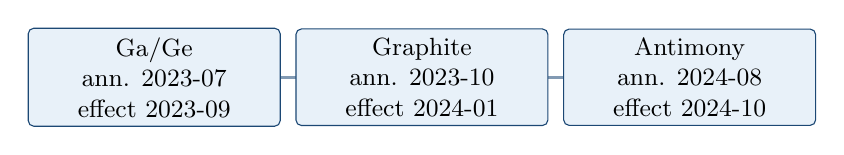
\begin{tikzpicture}[
    x=1cm,y=1cm,
    event/.style={draw=zjublue,fill=softblue,rounded corners=2pt,
      align=center,minimum width=3.2cm,minimum height=1.05cm,font=\small}
  ]
    \draw[very thick,zjublue!55] (0,0) -- (9.6,0);
    \node[event] at (1.4,0) {Ga/Ge\\ann. 2023-07\\effect 2023-09};
    \node[event] at (4.8,0) {Graphite\\ann. 2023-10\\effect 2024-01};
    \node[event] at (8.2,0) {Antimony\\ann. 2024-08\\effect 2024-10};
  \end{tikzpicture}
  \end{center}
\end{frame}

% Slide 3
\begin{frame}{Research Question and Argument}
  \Large
  \textbf{When do China's licensing-based critical-mineral export controls reduce importers' reliance on China?}

  \vspace{0.55cm}
  \large
  The effect should vary by:
  \begin{enumerate}
    \item product scope
    \item China exposure
    \item importer adjustment capacity
  \end{enumerate}

  \vfill
  \begin{beamercolorbox}[sep=0.85em,wd=\textwidth]{boxblue}
    \Large Legal control does not mechanically imply trade disruption.
  \end{beamercolorbox}
\end{frame}

% Slide 4
\begin{frame}{Data and Design}
  \begin{columns}[T,totalwidth=\textwidth]
    \begin{column}{0.46\textwidth}
      \large
      \textbf{Data}
      \begin{itemize}
        \item UN Comtrade monthly imports, 2019-01 to 2026-03.
        \item 53 reporters, 10 HS products.
        \item Each flow split: China source vs ROW.
        \item Outcome: observed monthly import value.
        \item Controls: alumina, manganese articles, inorganic acids.
      \end{itemize}
    \end{column}
    \begin{column}{0.50\textwidth}
      \large\textbf{Design: source-split PPML triple difference}

      \vspace{0.15cm}
      \begin{center}
      \begin{tikzpicture}[
        node distance=0.35cm,
        step/.style={draw=zjublue,fill=softblue,rounded corners=2pt,
          align=center,minimum width=5.3cm,minimum height=0.78cm,font=\small},
        arr/.style={-{Stealth[length=2mm]},thick,zjublue!75}
      ]
        \node[step] (a) {Treated product after control};
        \node[step,below=of a] (b) {China source vs ROW};
        \node[step,below=of b] (c) {Relative to untreated products};
        \draw[arr] (a) -- (b);
        \draw[arr] (b) -- (c);
      \end{tikzpicture}
      \end{center}

      \vspace{0.1cm}
      \[
      M_{ipst}=
      \exp\{\beta(Treated_p \times China_s \times Post_{kt})+\text{FE}\}
      \]

      \small
      \textbf{\(\beta<0\):} relative China-source import value falls.

      \smallnote{FE include importer-product, importer-source, product-month, source-month, product-source, and importer-month.}
    \end{column}
  \end{columns}
\end{frame}

% Slide 5
\begin{frame}{Product-Level Results: Selective Effects}
  \small
  \begin{tabularx}{\textwidth}{>{\raggedright\arraybackslash}p{0.36\textwidth}
      >{\raggedleft\arraybackslash}p{0.16\textwidth}
      >{\raggedright\arraybackslash}X}
    \toprule
    Product & Effect & Evidence \\
    \midrule
    Antimony oxides (HS 282580) & \(-81.5\%\) & clean central case \\
    Antimony metal (HS 8110) & \(-86.8\%\) & pretrends fail \\
    Antimony ores (HS 261710) & \(-98.9\%\) & sparse, descriptive \\
    Natural graphite (HS 2504) & \(-30.4\%\) & suggestive \\
    Ga/Ge bundle (HS 811292) & \(+19.3\%\) & no aggregate negative effect \\
    GeO$_2$/ZrO$_2$ (HS 282560) & \(+17.5\%\) & no aggregate negative effect \\
    \bottomrule
  \end{tabularx}

  \vspace{0.45cm}
  \begin{beamercolorbox}[sep=0.65em,wd=\textwidth]{boxblue}
    \small HS 282580: reporter \(p=0.002\); pretrend \(p=0.680\).
  \end{beamercolorbox}

  \smallnote{Exact product-assignment \(p\)-value floor = 0.25; reporter \(p\)-values are conditional diagnostics.}
\end{frame}

% Slide 6
\begin{frame}{Central Case: Antimony Oxides Event Study}
  \begin{columns}[T,totalwidth=\textwidth]
    \begin{column}{0.66\textwidth}
      \includegraphics[width=\textwidth]{figures/hs282580_eventstudy.pdf}
    \end{column}
    \begin{column}{0.31\textwidth}
      \large
      \begin{itemize}
        \item HS 282580: \(-81.5\%\) static effect.
        \item Pretrend \(p=0.680\).
        \item Post effect deepens over the first year.
        \item Cleanest reduced-form evidence of a binding licensing wedge.
      \end{itemize}
    \end{column}
  \end{columns}

  \smallnote{Coefficients are relative to m3; outcome is import value.}
\end{frame}

% Slide 7
\begin{frame}{Why Adjustment Capacity Matters}
  \large
  \(A_{ik}=\) pre-period China exposure \(\times\) ROW access

  \vspace{0.35cm}
  \begin{columns}[T,totalwidth=\textwidth]
    \begin{column}{0.48\textwidth}
      \begin{beamercolorbox}[sep=1.0em,wd=\textwidth]{boxgreen}
        \large\textbf{High \(A_{ik}\)}
        \vspace{0.25cm}

        {\Huge \(-87.4\%\)}

        \vspace{0.15cm}
        \normalsize \(p<0.001\), pretrend \(p=0.354\)
      \end{beamercolorbox}
    \end{column}
    \begin{column}{0.48\textwidth}
      \begin{beamercolorbox}[sep=1.0em,wd=\textwidth]{boxred}
        \large\textbf{Low \(A_{ik}\)}
        \vspace{0.25cm}

        {\Huge \(+103.1\%\)}

        \vspace{0.15cm}
        \normalsize \(p=0.035\), pretrend \(p=0.161\)
      \end{beamercolorbox}
    \end{column}
  \end{columns}

  \vfill
  \begin{beamercolorbox}[sep=0.7em,wd=\textwidth]{boxblue}
    \large This supports a source-switching interpretation for HS 282580.
  \end{beamercolorbox}
\end{frame}

% Slide 8
\begin{frame}{Discussion and Policy Implications}
  \large
  \begin{itemize}
    \item Do not infer disruption from legal announcements alone.
    \item HS-6 aggregation can hide controlled-item effects.
    \item Importer adjustment capacity shapes observed sourcing.
    \item Value data cannot separate prices, quantities, rerouting, or demand.
    \item Thesis extension: donor pool, partner-level ROW, exact-grade prices.
  \end{itemize}

  \vfill
  \begin{beamercolorbox}[sep=0.9em,wd=\textwidth]{boxblue}
    \Large The result is not ``China controls everything''; it is ``some licensing controls visibly shift sourcing, under specific product and importer conditions.''
  \end{beamercolorbox}
\end{frame}

\setbeamertemplate{footline}{}
\appendix

% Optional references slide
\begin{frame}[noframenumbering]{Selected References}
  \small
  \begin{itemize}
    \item Farrell and Newman (2019, 2023)
    \item Bown (2020); Bown and Wang (2024)
    \item International Energy Agency (2025)
    \item U.S. Geological Survey (2026)
    \item MOFCOM/GAC export-control announcements
    \item Roth (2022)
  \end{itemize}
\end{frame}

% Optional backup slide
\begin{frame}[noframenumbering]{Backup: Robustness for HS 282580}
  \large
  \begin{tabular}{lr}
    \toprule
    Check & Effect \\
    \midrule
    Baseline & \(-81.5\%\) \\
    Truncate at 2025-12 & \(-79.6\%\) \\
    Reported-only sample & \(-81.7\%\) \\
    Donor-pool range & \(-81.0\%\) to \(-83.6\%\) \\
    Leave-one-reporter range & \(-63.6\%\) to \(-84.4\%\) \\
    \bottomrule
  \end{tabular}

  \vspace{0.5cm}
  \normalsize All leave-one-reporter estimates stay below \(-50\%\).
\end{frame}

\end{document}
